% Chapter Template

\chapter{Disseny} % Main chapter title

\label{Disseny} % Change X to a consecutive number; for referencing this chapter elsewhere, use \ref{ChapterX}

Aquest projecte consta del desenvolupament d'una aplicació \textit{Android}, per aquest motiu l'arquitectura ha d'adaptar-se a les bones pràctiques d'aquesta plataforma.\\

El sistema separa clarament els conceptes en activitats diferents. Com que es tracta d'un dispositiu mòbil, aquestes activitats només són un llaç entre el sistema operatiu i l'aplicació, per tant, no sempre les controlem i en el cas que el dispositiu mòbil necessiti memòria pot eliminar l'activitat. Si separem els conceptes en activitats diferents minimitzem les dependències.

\section{Arquitectura}

Per al desenvolupament d'aquest projecte s'ha obtat per utilitzar l'arquitectura que proporciona la plataforma \textit{Android} per defecte. Aquesta consta d'un conjunt d'activitats que fan servir un model i controlen la interfície. En l'Activitat, només hi ha de constar el codi que faci de vincle entre el model i la vista, per aquest motiu, per tal de dur a terme tots els processos que es necessiten per obtenir la informació adequada s'ha dissenyat un servei (figura 8.1).

\begin{figure}[!h]
\centering
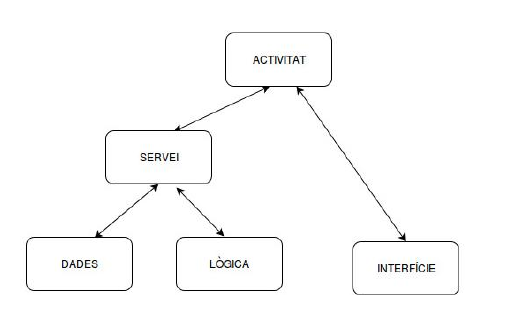
\includegraphics[scale=0.65]{Figures/ArquitecturaSistema.jpg}
\caption{Arquitectura de l'aplicació.}
\end{figure}

\begin{itemize}

\item[]{\textbf{Activitat}}\\
El sistema implementa una activitat per a cada funcionalitat diferent, d'aquesta manera, com s'ha exposat anteriorment, minimitzem les dependències i garantim més fiabilitat. No existeix un controlador que goberni les activitats sinó que es cada activitat que sap en tot moment amb qui s'ha de comunicar i qui pot ser que es comuniqui amb ella.\\

\item[]{\textbf{Servei}}\\
Des de qualsevol activitat es pot accedir a un servei per tal d'obtenir dades que es volen utilitzar per mostrar-les a l'usuari. En la figura 8.2 es pot apreciar una part de l'estructura dels serveis, es declara un servei per cada temàtica, dins el servei es dur a terme les operacions que convinguin utilitzant les dades guardades en els repositoris.

\begin{figure}[!h]
\centering
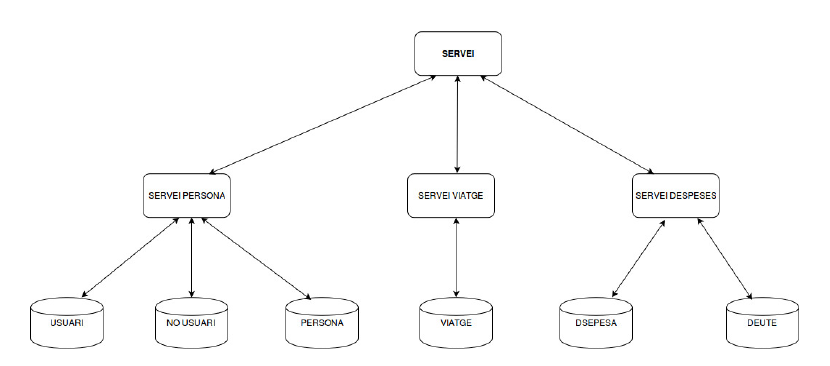
\includegraphics[scale=0.70]{Figures/EstructuraServeis.jpg}
\caption{Estructura dels serveis.}
\end{figure}

\item[]{\textbf{Dades}}\\
Es tenen en compte dos tipus de fonts de dades, les que guardem i consultem de la base de dades i les que obtenim de les consultes a serveis externs. Des del punt de vista de l'activitat, no hi ha cap diferencia en accedir-hi. \\
En el cas de les dades guardades a la base de dades, la qual està en el núvol, s'utilitzen uns repositoris per tal de tenir les dades en local. Hi ha un repositori per cada tipus d'entitat a la base de dades. En la figura 8.3 es pot apreciar l'accés des de l'activitat a la base de dades.\\
Pel que fa a les consultes a serveis externs no s'utilitzen respositoris, des del servei es fa una crida directament a la API corresponent per tal d'obtenir les dades i és al mateix servei on es tracten i es torna el resultat desitjat a l'activitat (figura 8.4).


\begin{figure}[!h]
\centering
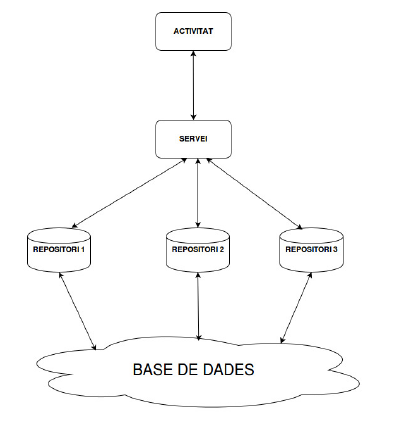
\includegraphics[scale=0.6]{Figures/AccesBD.jpg}
\caption{Accés a les dades.}
\end{figure}

\begin{figure}[!h]
\centering
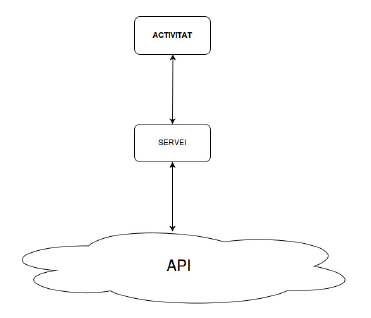
\includegraphics[scale=0.7]{Figures/AccesAPI.jpg}
\caption{Accés a serveis externs.}
\end{figure}

\clearpage

\end{itemize}


\subsection{Patrons}

Es va tenir en compte l'arquitectura Model-View-Controller però això provoca que s'hagi de trencar el gran acomplament que ofereix la plataforma Android entre el controlador i la vista. Per aquest motiu es va decidir decantar el disseny de l'arquitectura del projecte cap a l'estructura explicada en l'apartat anterior. 

\subsection{Tecnologies utilitzades}
\begin{itemize}
\item[]{\textbf{Android}}\\
És el sistema operatiu per a dispositius mòbils amb pantalla tàctil més utilitzat. Actualment l'utilitzen des de telèfons inteligens i tables, fins a rellotges de nova generació, televisors i automòbils. És un projecte de codi obert recolçat per Google des del 2008. El desenvolupament d'aplicacions es fa habitualment en llenguatge Java i es diposa d'un SDK (Software Development Kit) que es pot descarregar gratuïtament des de la pàgina web oficial.\\

\item[]{\textbf{JSON}}\\
JavaScript Object Notation és el nom que rep una forma d'estructurar les dades per, posteriorment, ser enviades entre dispositius o per la xarxa. Es l'alternativa a XML en termes de llenguatge marcat i s'acostuma a utilitzar en les aplicacions Android per la comunicació amb el servidor o serveis externs.\\

\item[]{\textbf{Firebase}}\\
Firebase ofereix una base de dades en temps real com a servei. Aquest servei ofereix als desenvolupadors una API que permet guardar dades al núvol de les seves aplicacions. La companyia ofereix al client diverses llibreries per tal de facilitar la integració amb Android, iOS, Java i d'altres aplicacions.

\end{itemize}

\clearpage

\section{Capa de presentació}
\begin{itemize}

\item[]{\textbf{Iniciar sessió}}\\
El procés d'identificació de l'usuari es dur a terme a través de Google, per tant, l'usuari no es registra al nostre sistema sinó que utilitza les credencials del seu compte de Google per tal d'identificar-se.



\begin{figure}[!h]
\centering
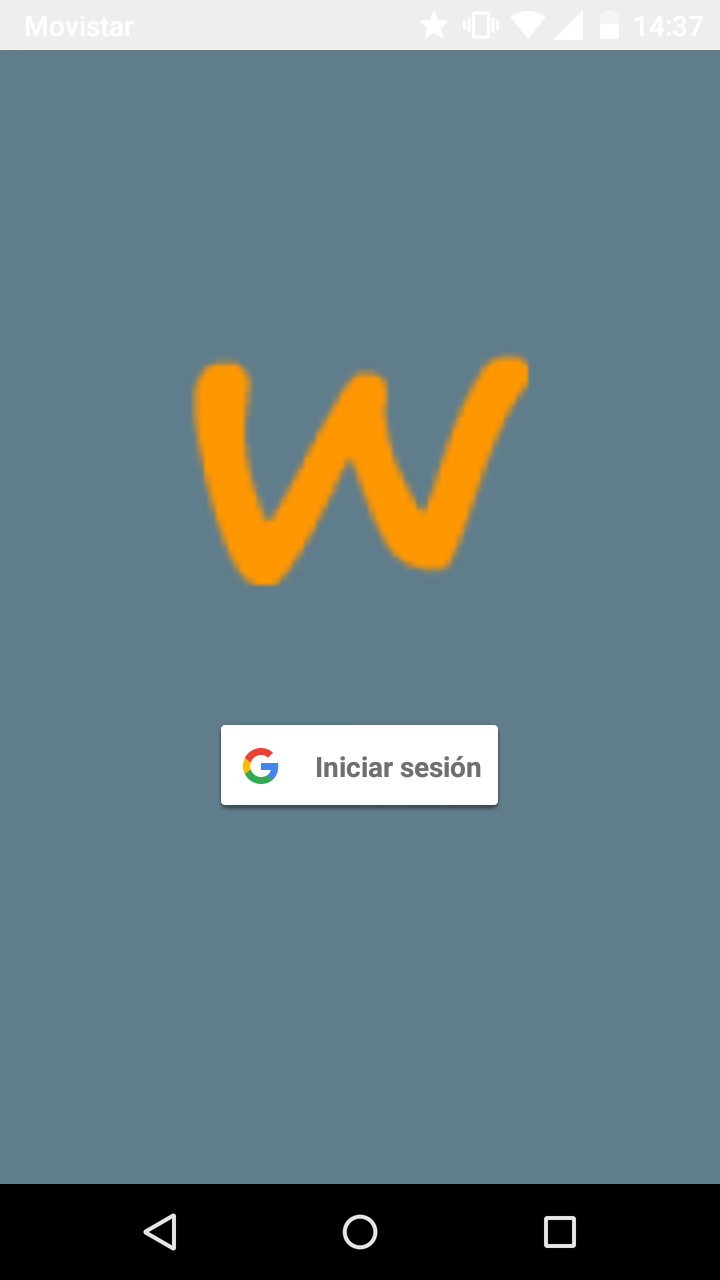
\includegraphics[scale=0.15]{Figures/initSesion.png}
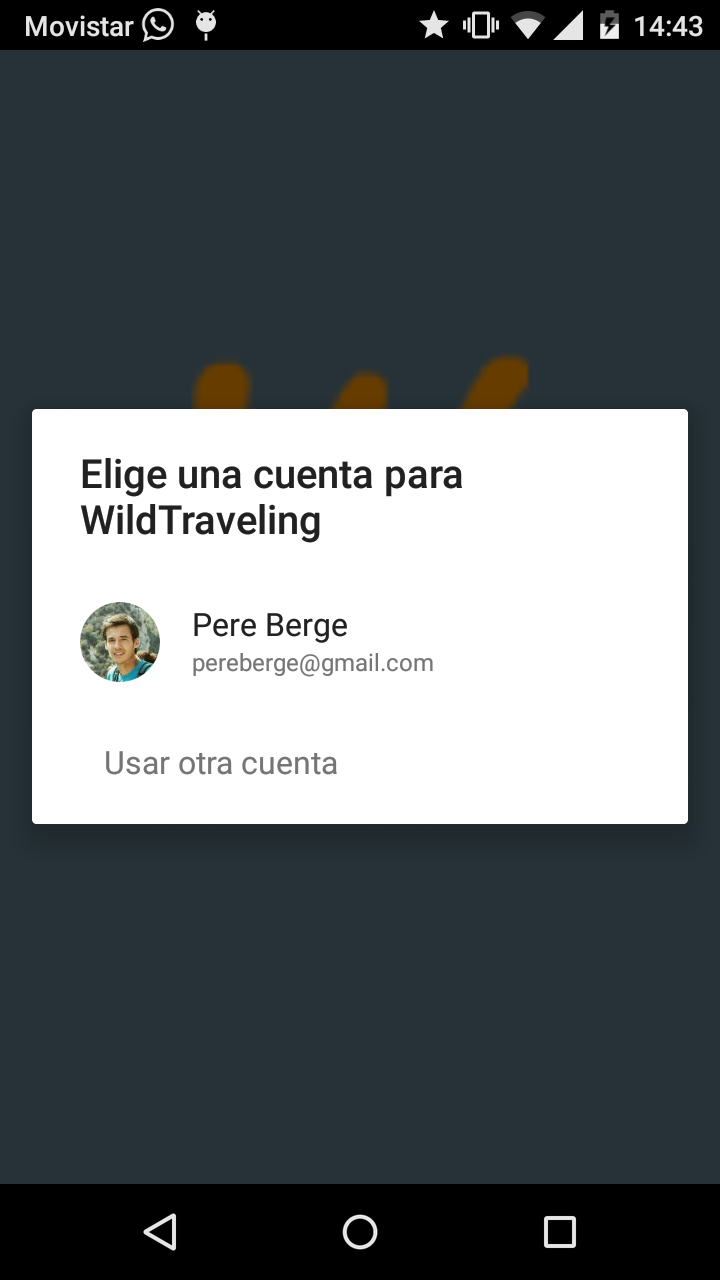
\includegraphics[scale=0.15]{Figures/TriarComte.png}
\caption{Inici de sessió}
\end{figure}



\item[]{\textbf{Consultar llista de viatges}}\\
A la pantalla de consultar viatges es mostra la llista de viatges de lúsuari. Si l'usuari selecciona qualsevol viatge l'aplicació el redigirà a la pantalla de consulta de viatge. També hi ha l'opció de crear un nou viatge.

\begin{figure}[!h]
\centering
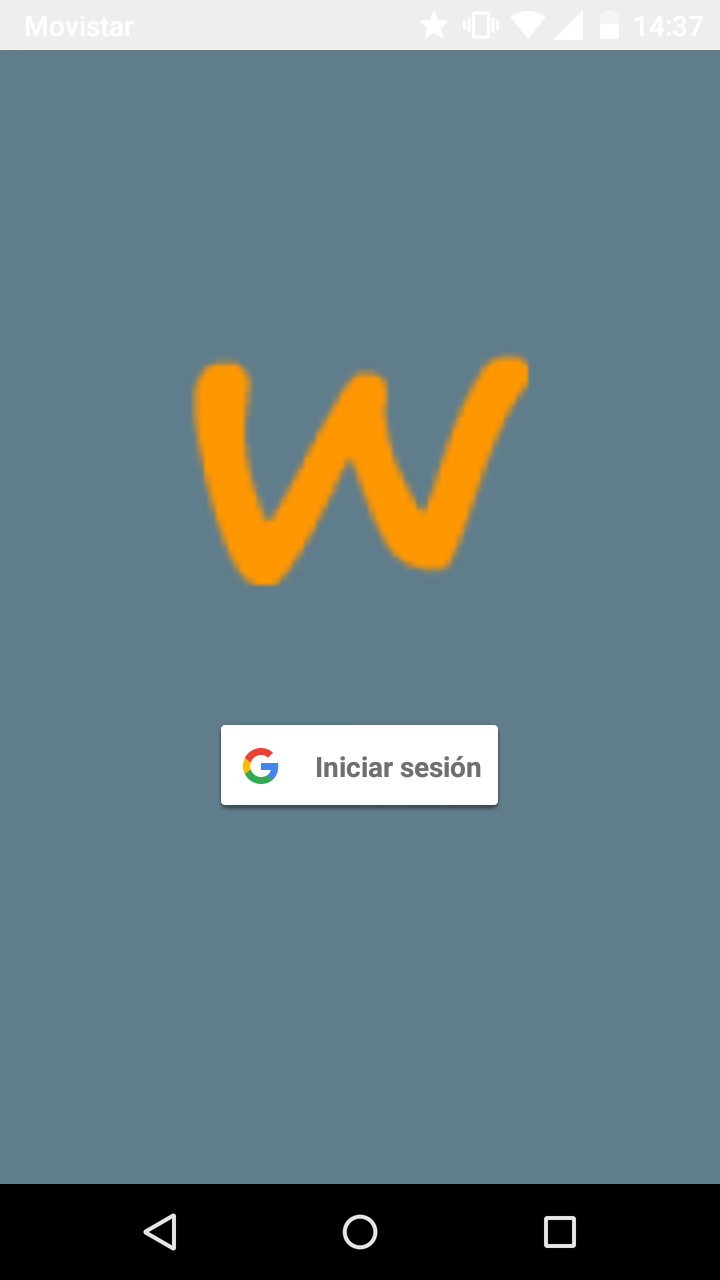
\includegraphics[scale=0.15]{Figures/initSesion.png}
\caption{Inici de sessió}
\end{figure}

\item[]{\textbf{Crear viatge}}\\
En aquesta pantalla és on s'introdueixen totes les dades d'un nou viatge com el nom, el destí, les dates i els participants. A més, el sistema li pregunta sobre el seu estil de viatjar i demana que li introdueixi les dades d'un contacte d'emergència. Un cop creat el viatge, l'aplicació redirigeix l'usuari a la pantalla de consultar viatge.

\clearpage

\begin{figure}[!h]
\centering
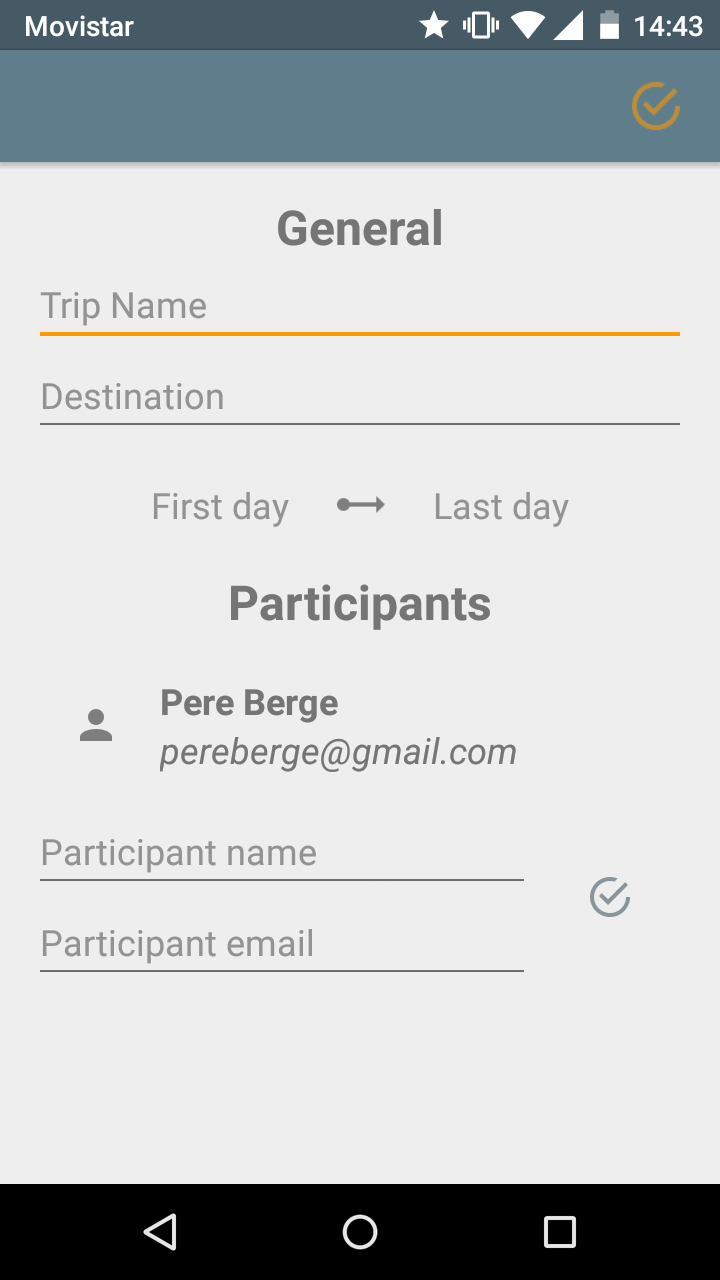
\includegraphics[scale=0.15]{Figures/cerarViatge.png}
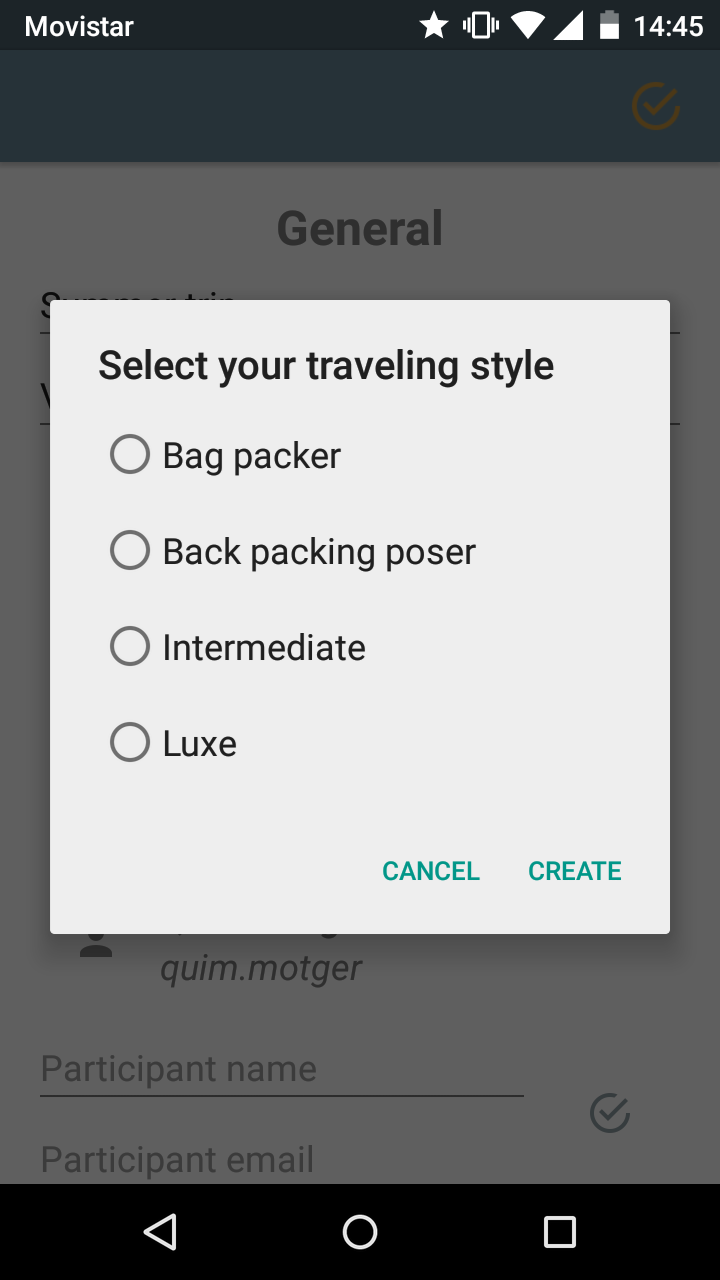
\includegraphics[scale=0.15]{Figures/style.png}
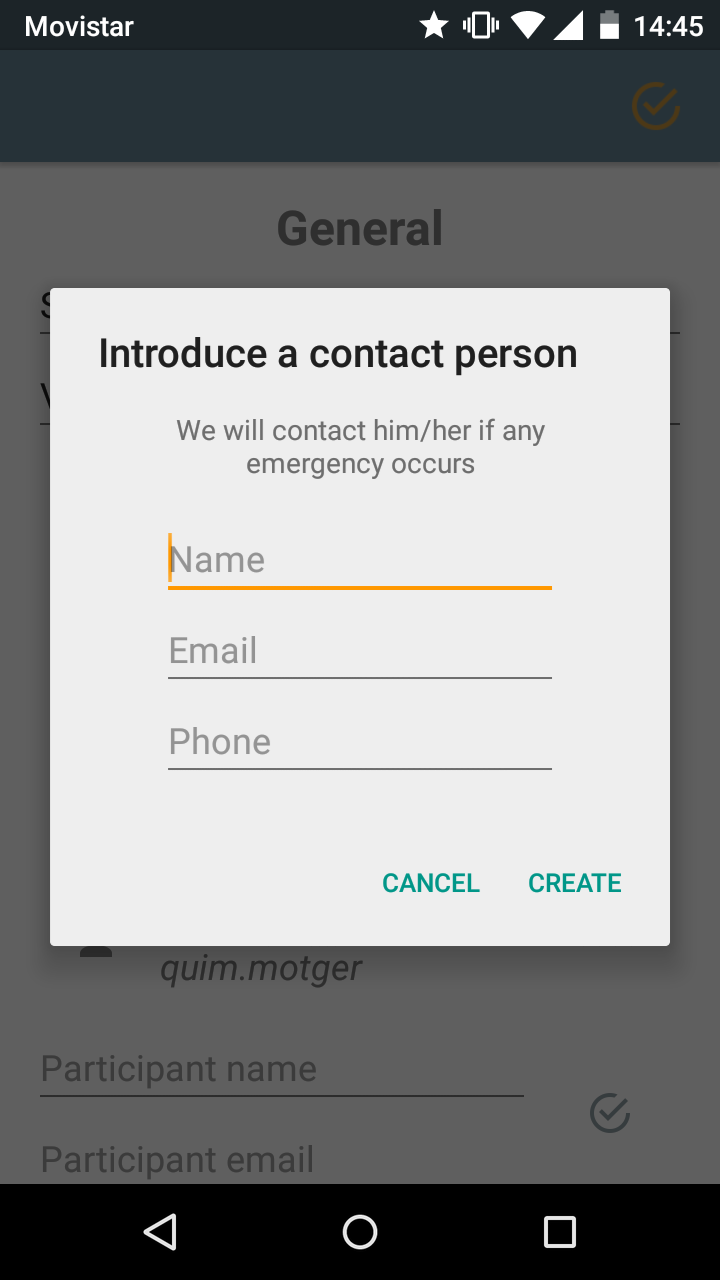
\includegraphics[scale=0.15]{Figures/emergencyContact.png}
\caption{Crear viatge}
\end{figure}

\item[]{\textbf{Consultar viatge}}\\
La pantalla on es mostra tota la informació del viatge: nom, destí, dates i participants. A més, és la pantalla des d'on es pot accedir a totes les funcionalitats nombrades en apartats anteriors i permet eliminar el viatge.

\begin{figure}[!h]
\centering
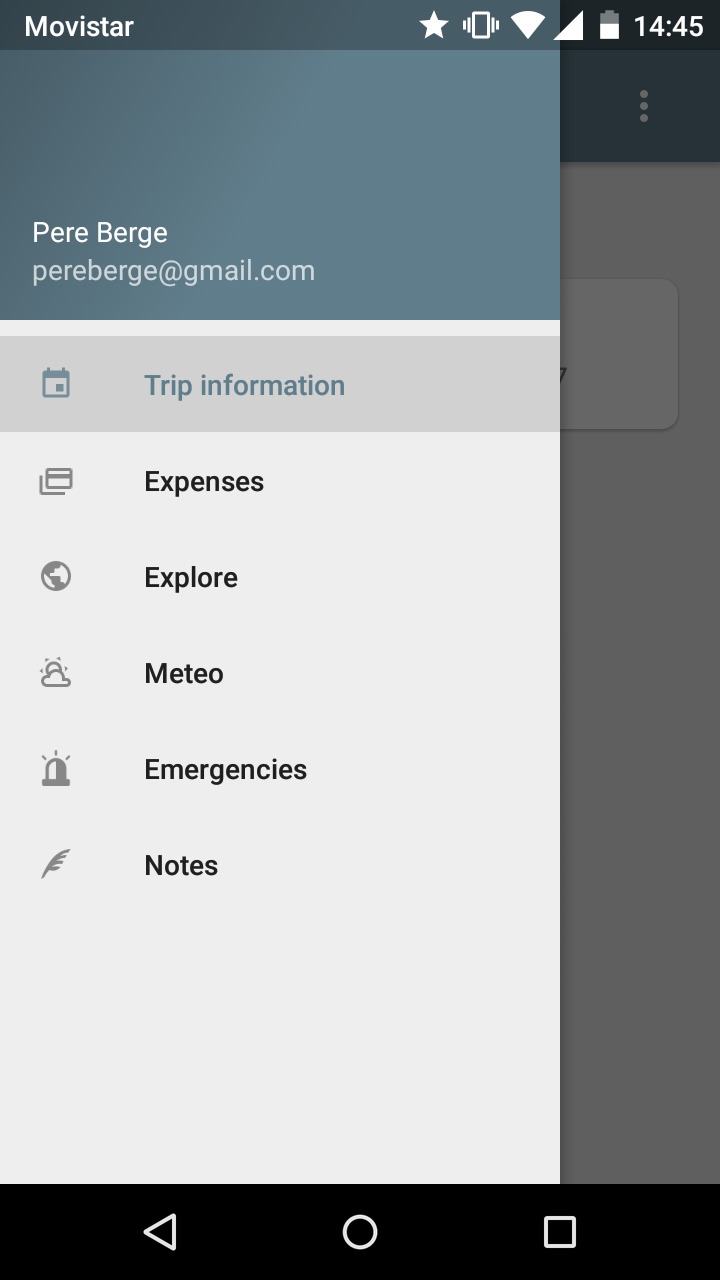
\includegraphics[scale=0.15]{Figures/Drawer.png}
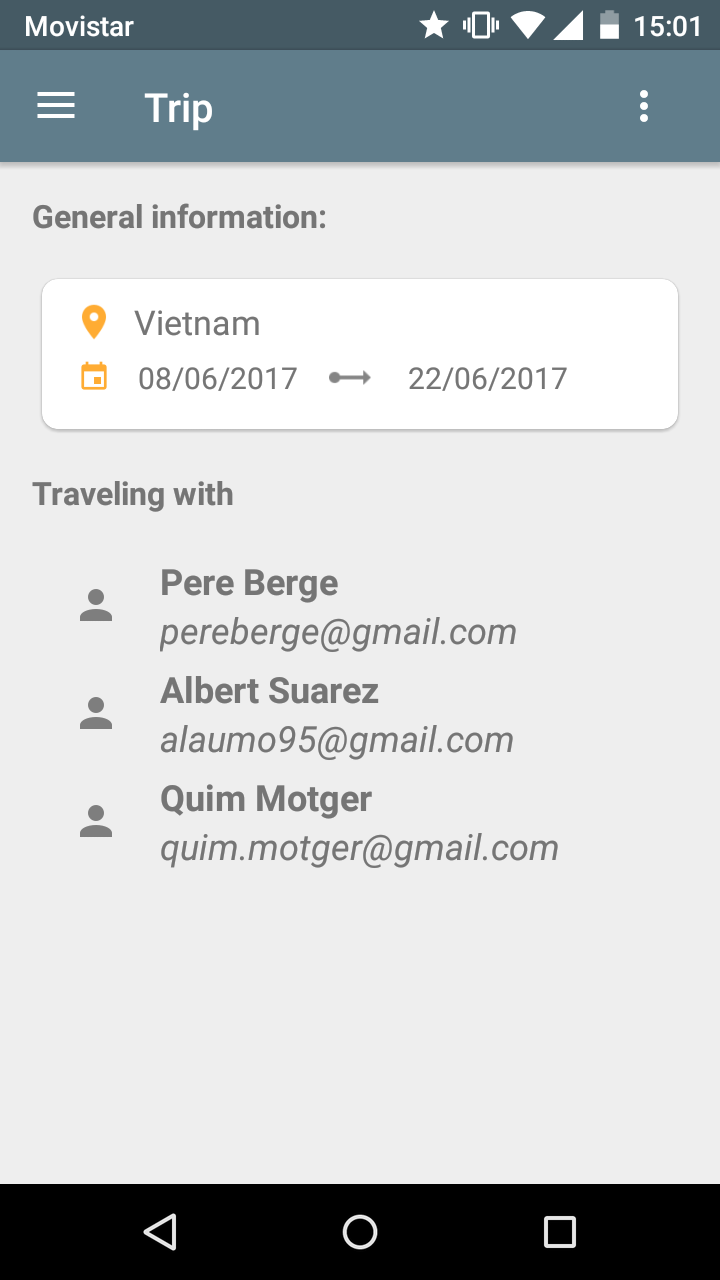
\includegraphics[scale=0.15]{Figures/getTrip.png}
\caption{Consultar viatge}
\end{figure}

\item[]{\textbf{Consultar llista de despeses}}\\
La pantalla de consultar despeses és on es poden veure totes les despeses del viatge i la quantitat total gastada. Si l'usuari selecciona una despesa el sistema el redirigeix a la pantalla de consultar despesa. A més, l'usuari també té l'opció de crear-ne una de nova, fet que el portarà a la pantalla de crear despesa.

\clearpage

\begin{figure}[!h]
\centering
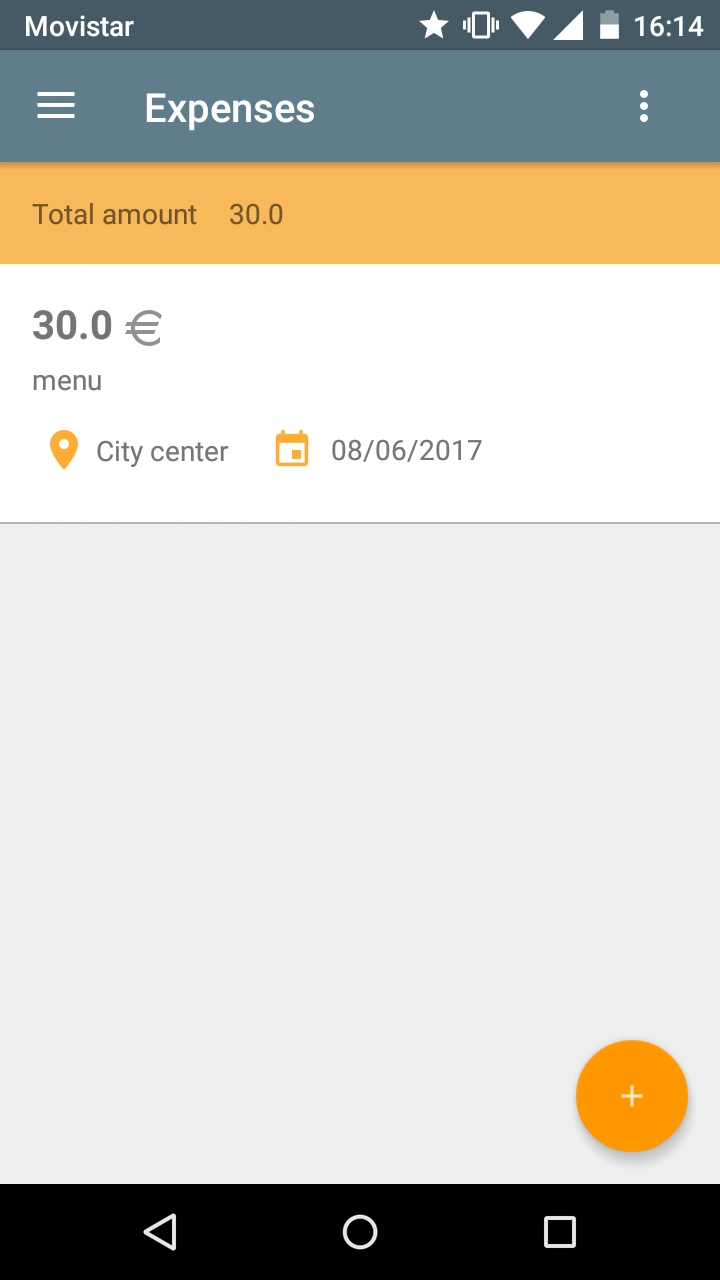
\includegraphics[scale=0.15]{Figures/llistaDespeses.png}
\caption{Llista despeses}
\end{figure}

\item[]{\textbf{Crear despesa}}\\
En la pantalla crear despesa l'usuari introdueix les dades de la nova despesa com el motiu, la quantitat a pagar, la localització i si ha pagat una part a un company de viatge. Un cop creada la despesa el sistema redirigeix l'usuari a la pantalla de consultar despesa.

\begin{figure}[!h]
\centering
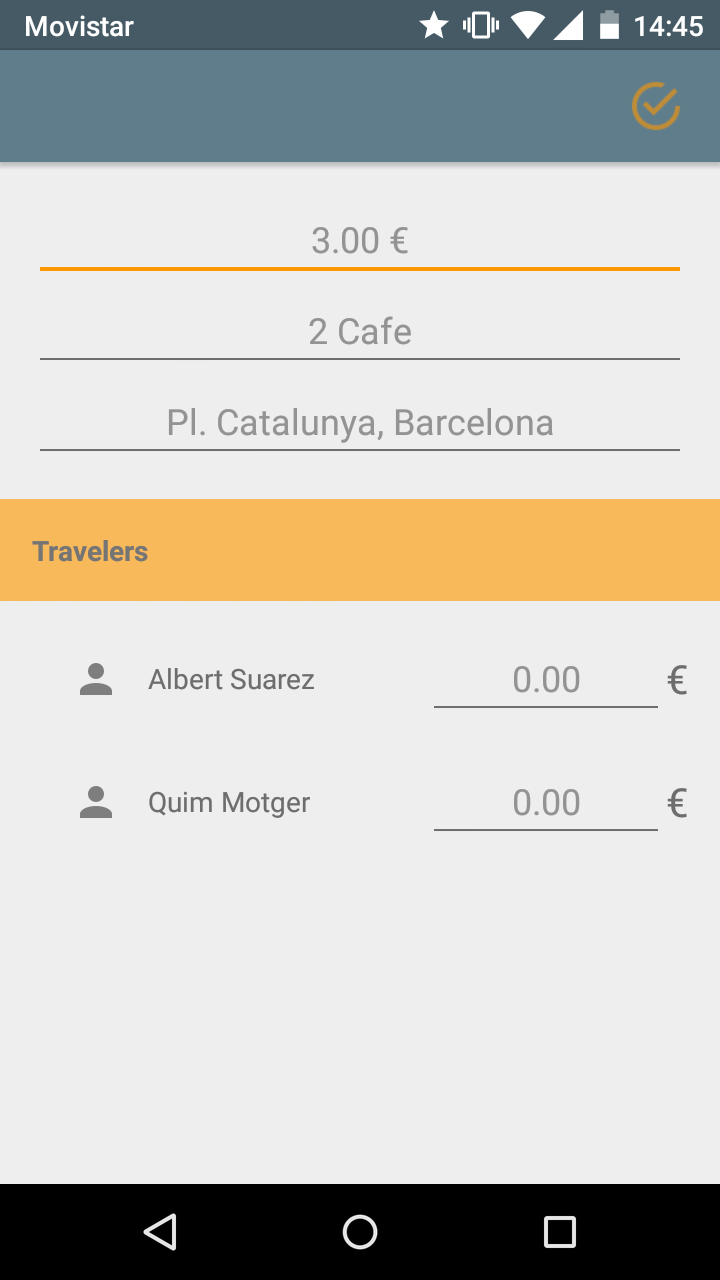
\includegraphics[scale=0.15]{Figures/crearDespesa.png}
\caption{Crear despesa}
\end{figure}

\item[]{\textbf{Consultar despesa}}\\
En la pantalla de consultar despesa l'usuari pot veure tota la informació de les despeses i té l'opció de marcar un deute com a pagat, modificar la despesa o eliminar-la. En el cas que l'usuari seleccioni modificar despesa el sistema el redirigeix a la pantalla de modificació de despesa, per l'altra banda, si decideix eliminar la despesa, el sistema el redirigeix a la pantalla de consultar llista de despeses.

\clearpage

\begin{figure}[!h]
\centering
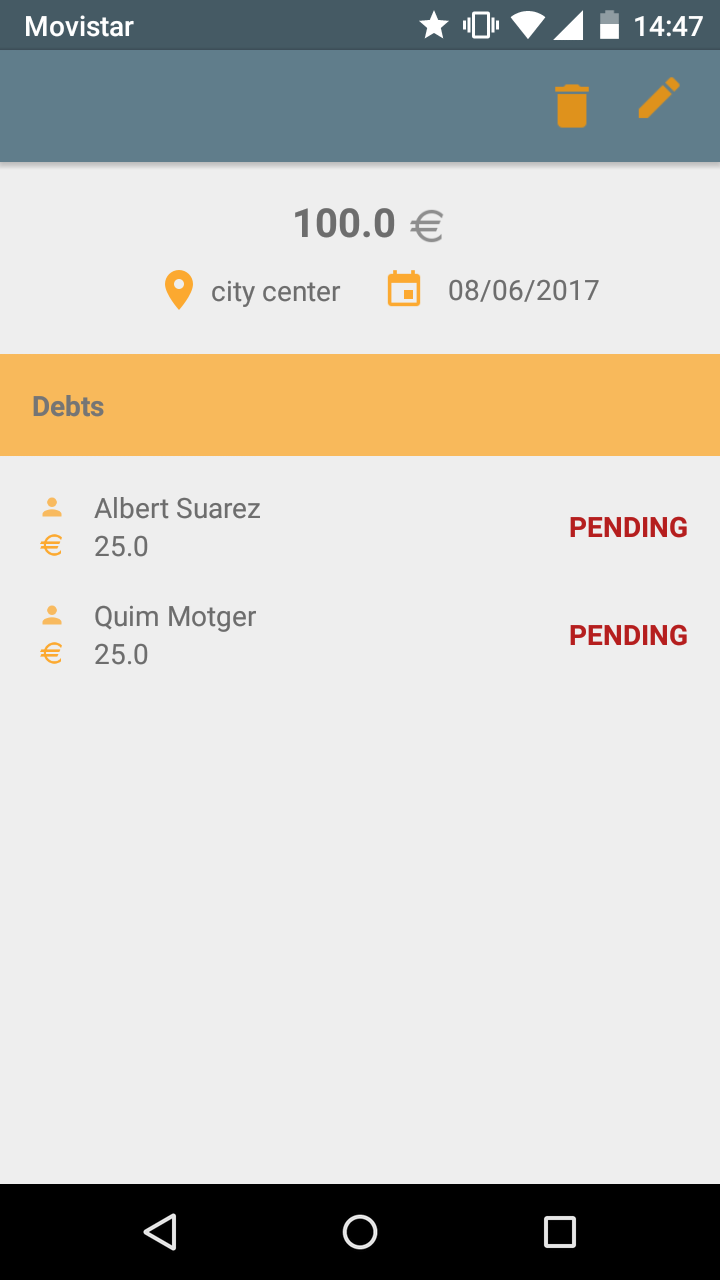
\includegraphics[scale=0.15]{Figures/consultarDespesa.png}
\caption{Consultar despesa}
\end{figure}

\item[]{\textbf{Modificar despesa}}\\
En la pantalla de modificar despesa l'usuari pot modificar totes les dades d'una despesa. Quan comfirma la modificació el sistema el redirigeix la pantalla de consultar despesa.



\begin{figure}[!h]
\centering
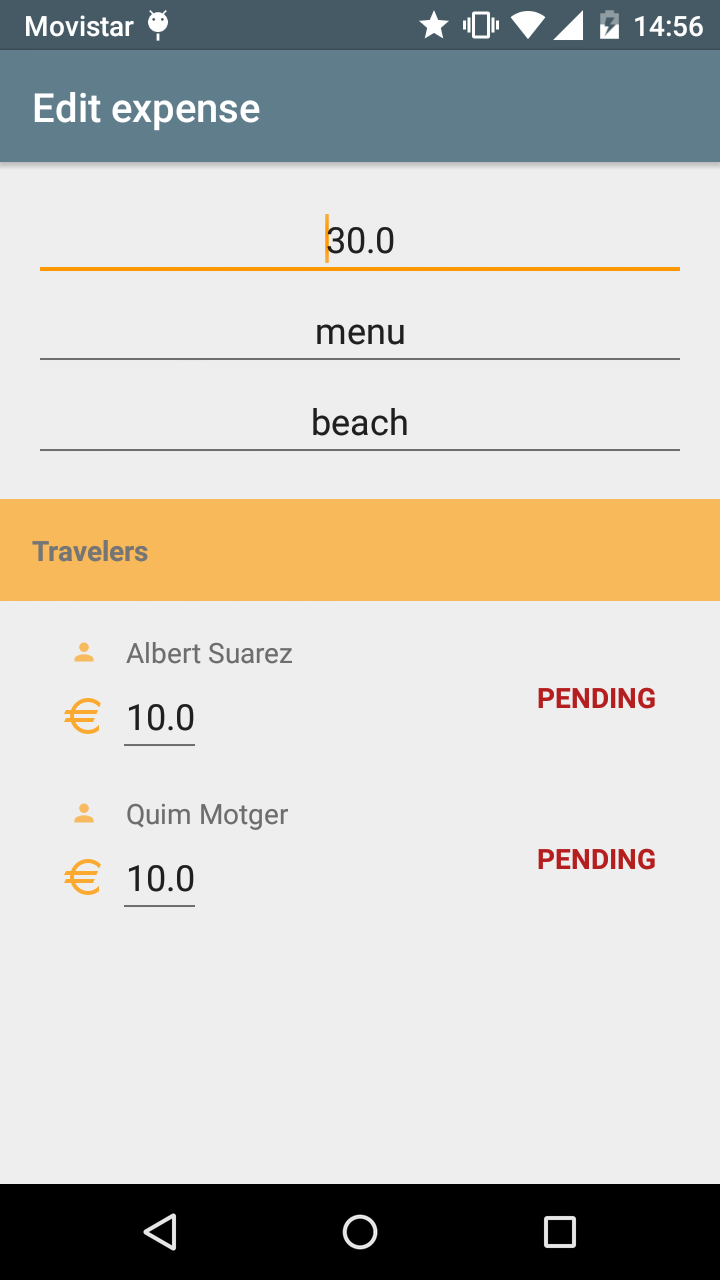
\includegraphics[scale=0.15]{Figures/modificarDespesa.png}
\caption{Modificar despesa}
\end{figure}

\item[]{\textbf{Cerca lloc d'interés}}\\
En la pantalla de cerca lloc d'interés l'usuari pot seleccionar què vol buscar d'entre les possibilitats proposades i a quin lloc ho vol buscar. Si el lloc on ho vol buscar queda buit, es cercaran els resultats tenint en compte la localització de l'usuari en el moment de la cerca. Si no es troben resultats o es necessita activar el GPS s'informarà a l'usuari, d'altra banda, si la cerca es dur a terme satisfactoriament el sistema redirigirà l'usuari a la pantalla de llista de resultats de cerca.

\clearpage

\begin{figure}[!h]
\centering
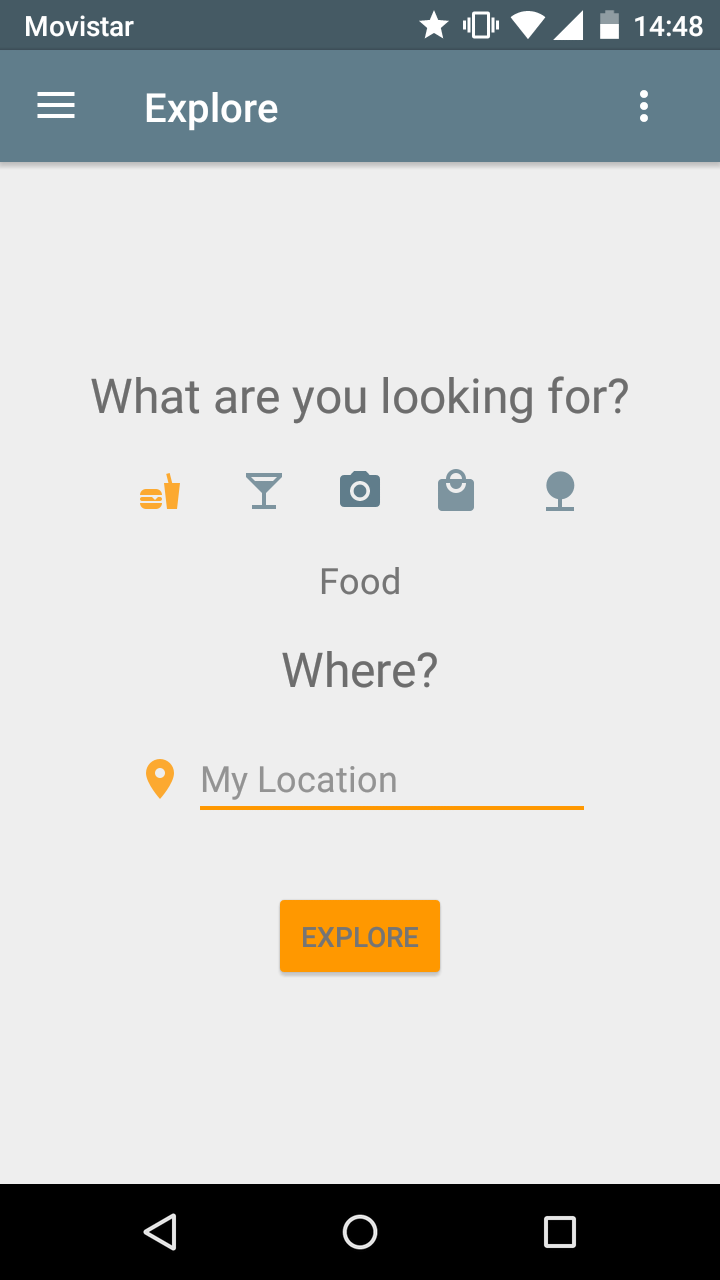
\includegraphics[scale=0.15]{Figures/cerca.png}
\caption{Cerca de llocs d'interès}
\end{figure}

\item[]{\textbf{Consultar llista de resultats de cerca}}\\
És la pantalla on es veuen les resultats de la cerca, aquests estan ordenats per l'estil de viatjar de l'usuari. Per a cada item trobat es pot consultar el nom, la localització i, en cas que n'hi hagi, el nivell de preus de l'establiment. Quan l'usuari selecciona un resultat de la cerca el sistema el redirigeix a la pantalla de consultar ruta.


\begin{figure}[!h]
\centering
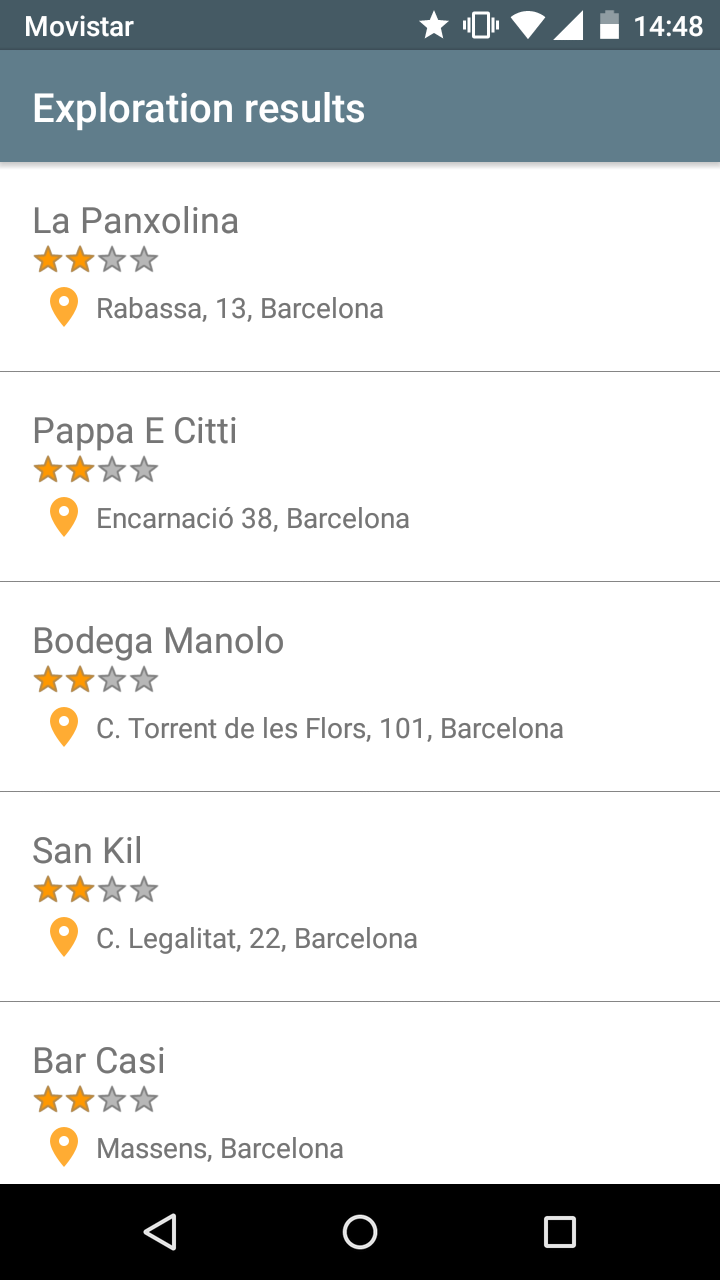
\includegraphics[scale=0.15]{Figures/resultatsCerca.png}
\caption{Resultats de cerca}
\end{figure}



\item[]{\textbf{Consultar ruta}}\\
En la pantalla de consultar ruta, l'usuari pot veure diverses opcions de ruta des d'on s'ha fet la cerca fins al punt seleccionat. A més, pot consultar la ruta en cotxe, transport públic i a peu, per a cada modalitat es poden veure paràmetres com la distància en quilòmetres i el temps que tardarà en arribar-hi. Si l'usuari prem sobre una de les rutes, l'aplicació li dona l'opció de consultar la ruta exacta utilitzant, en el cas que l'usuari la tingui instalada, l'aplicació Google Maps. Per últim, l'usuari té l'opció de consultar la ruta inversa.

\clearpage

\begin{figure}[!h]
\centering
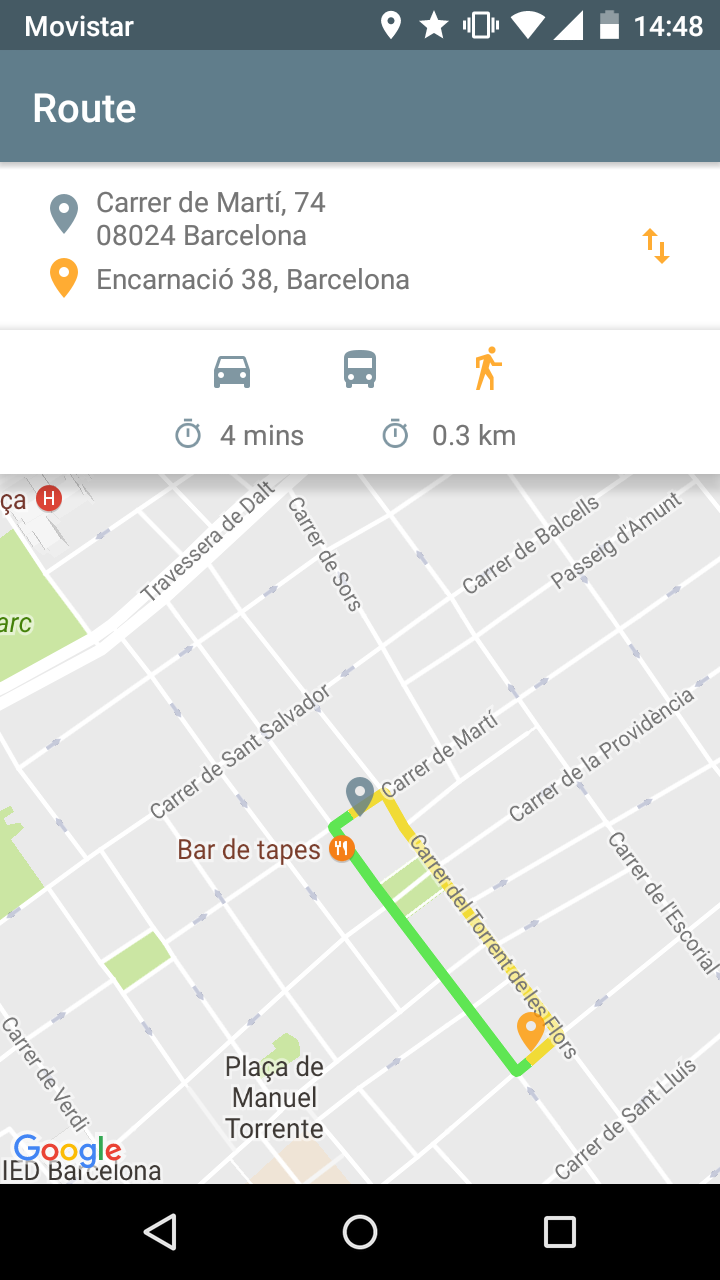
\includegraphics[scale=0.15]{Figures/ruta.png}
\caption{Consultar ruta}
\end{figure}

\item[]{\textbf{Consultar previsió metereològica}}\\
En la pantalla de consultar previsió metereològica es pot veure la metereologia del dia actual amb paràmetre com la temperatura màxima i mínima, el percentatge de possibilitat de pluja, la velocitat del vent o la descripció del cel. A més, l'usuari també pot consultar la previsió fins a sis dies vista.


\begin{figure}[!h]
\centering
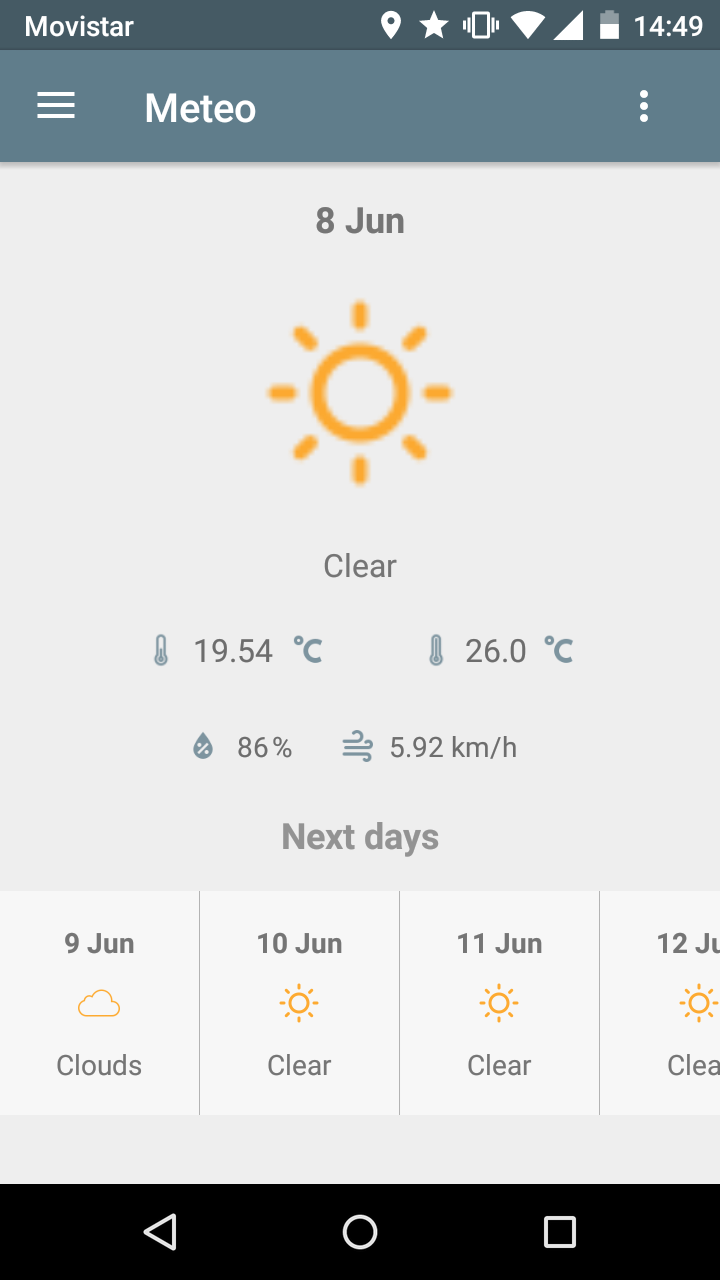
\includegraphics[scale=0.15]{Figures/meteo.png}
\caption{Previsió metereològica}
\end{figure}

\item[]{\textbf{Emergències}}\\
En la pantalla d'emergències l'usuari té tres opcions. La primera és realitzar una trucada al telèfon d'emergències del país on estigui, si selecciona aquesta opció el sistema el redirigirà a la pantalla de trucades del seu dispositiu mòbil. La segona opció es tracta de realitzar una trucada al seu propi contacte d'emergències, en aquest cas també se'l redirigirà a la pantalla de trucades del seu dispositiu mòbil. Per últim, té l'opció de seleccionar l'opció d'obtenir la ruta a l'hospital més proper, en aquest cas se'l redirigirà a la pantalla de consultar ruta.

\begin{figure}[!h]
\centering
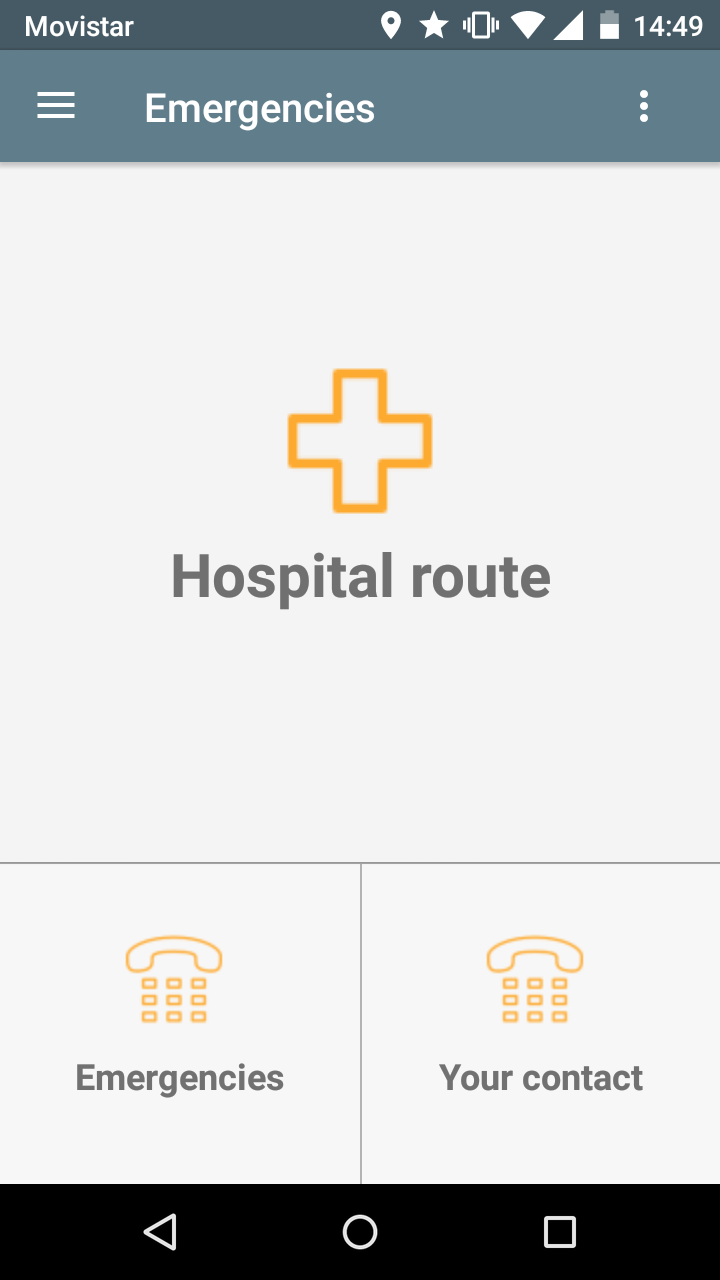
\includegraphics[scale=0.15]{Figures/emergencies.png}
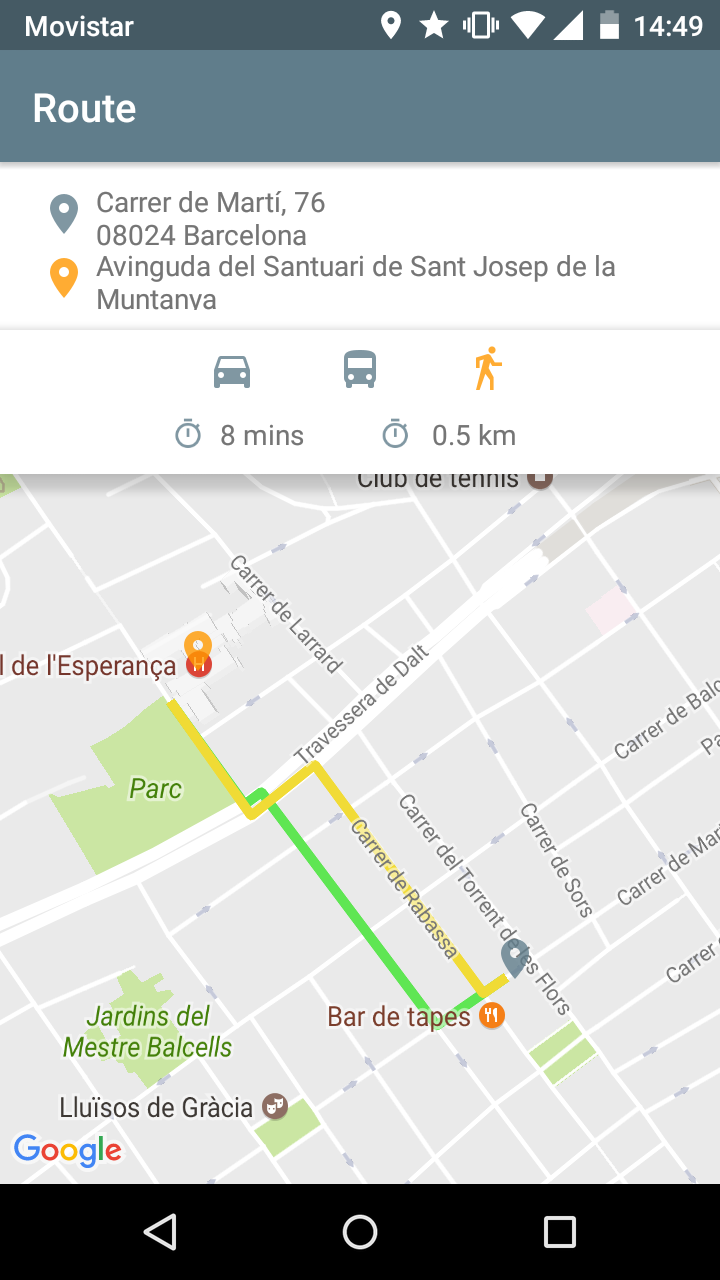
\includegraphics[scale=0.15]{Figures/hospital.png}
\caption{Gestió d'emergències}
\end{figure}

\end{itemize}

%\section{Canvis en les restriccions}

\section{Diagrama de classes de disseny}

\section{Model de dades}

En aquest apartat s'explica el model de dades utilitzat per desenvolupar el projecte. La base de dades que s'ha utilitzat és un base de dades no relacional de tipus \textit{key-value}. Per tal de modelar les dades, s'han seguit les bones pràctiques de la tecnologia utilitzada \textit{Firebase}.\\

Les dades del projecte es guarden en una direcció concreta, existeix un node pare del projecte des d'on pengen totes les dades. A partir d'aquest node pare es creen nodes per a cada tipus de dades diferent a guardar. D'aquests subnodes en pengen llistes clau-valor amb totes les dades emmagatzemades d'aquell tipus concret (figura 8.5). En els manuals de \textit{Firebase} es dona molta importància a l'organització de la base de dades tal com s'ha explicat en aquest paràgraf.\\

\begin{figure}[!h]
\centering
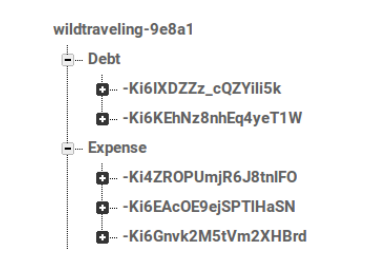
\includegraphics[scale=1.00]{Figures/EstructuraBD.jpg}
\caption{Estructura base de dades.}
\end{figure}


Per a cada clau tenim un valor, aquest valor conté tots els atributs de l'entitat guardada. Per tal d'evitar emmagatzemar informació duplicada guardant altres entitats dins d'entitats, quan es necessita afrontar aquest cas el que es fa és guardar només la clau (figura 8.6).


\begin{figure}[!h]
\centering
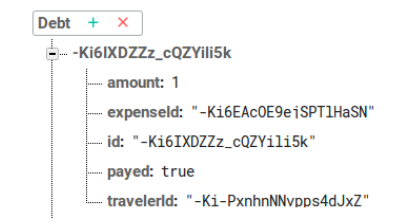
\includegraphics[scale=1.00]{Figures/DebtBD.jpg}
\caption{Solució per no duplicar informació.}
\end{figure}

Aquest sistema, per tal de ser el màxim eficient, utilitza índexs a l'hora d'accedir a un valor a través de la seva clau.

\section{Diagrames de seqüència}
